\documentclass[11pt, A4paper, english]{article}
\usepackage{amsfonts}
\usepackage{amsmath}
\usepackage{amssymb}
\usepackage{amsthm}
\usepackage{babel}
\usepackage{color}
\usepackage{float}
\usepackage[T1]{fontenc}
\usepackage{graphicx}
\usepackage[colorlinks]{hyperref}
\usepackage[utf8]{inputenc}
\usepackage{listings}
\usepackage{textcomp}
\usepackage[style=ieee]{biblatex}
\usepackage{tabularx}

\addbibresource{bibliography.bib}

\definecolor{dkgreen}{rgb}{0, 0.6, 0}
\definecolor{gray}{rgb}{0.5, 0.5, 0.5}
\definecolor{daynineyellow}{rgb}{1.0, 0.655, 0.102}
\definecolor{url}{rgb}{0.1, 0.1, 0.4}

\lstset{frame=tb,
	language=csh,
	aboveskip=3mm,
	belowskip=3mm,
	showstringspaces=false,
	columns=flexible,
	basicstyle={\small\ttfamily},
	numbers=none,
	numberstyle=\tiny\color{gray},
	keywordstyle=\color{blue},
	commentstyle=\color{daynineyellow},
	stringstyle=\color{dkgreen},
	breaklines=true,
	breakatwhitespace=true,
	tabsize=3
}

\lstset{inputpath="C:/Users/Torstein/Documents/skole/USN/IIA2017/Assignment 5"}
\graphicspath{{C:/Users/Torstein/Documents/USN/IIA2017/Assignment 5/}}
\hypersetup{colorlinks = true, linkcolor = black, urlcolor=url}

\author{Torstein Solheim Ølberg | 263054}
\title{Assignment 5 in IIA2017}



%\lstinputlisting{Filnavn! type kodefil}. Use [linerange=0-73] or [linerange=73-] to crop
%\includegraphics[width=12.6cm, height=8cm]{Filnavn! type png}



\begin{document}
\maketitle
\clearpage

\tableofcontents
\clearpage

	\section{Introduction}
MyCompany AS has decided to enter the contest \cite{task} outlined by Industrial Production Company to produce a datalogging and monitoring system proff of consept. As the task describes, the system should consist of at least an SQL server database, a datalogging system and a data monitoring system. For this purpose, MyCompany has decided to use Microsoft SQL Server to host the server locally, LabVIEW to develop the Datalogging system and C sharp using Microsoft Visual Studio to develop the Monitoring system. \\
In LabVIEW, the Database Connectivity Toolkit package \cite{NIDB} is used to connect to, perform actions with and close the connection to the SQL server. For the SQL server, erwin Database Modeler \cite{erwin} is used to both set up the general structure of the database and to produce a documentation diagram for the database. Finally, the Chart package for C sharp is used to create plots for the monitoring program. \\
This report will present the SQL server, then the logging system. The resulting system will be discussed and any improvements will be suggested, before a conclusion is drawn. The documentation diagrams for the server and the datalogging system can be found in Appendix A.

	\section{Results}
		\subsection{SQL Server}
The SQL server is called SQLEXPRESS and the database is called Datalogging and Monitoring System. It can be accessed via the connection string "{Server=localhost\\SQLEXPRESS;Database=Datalogging and Monitoring System;Trusted\_Connection=True;" on the computer used for its development. As figure \ref{SQLDiagram} shows, the SQL database consists of four tables, each saving different information.
			\begin{figure}
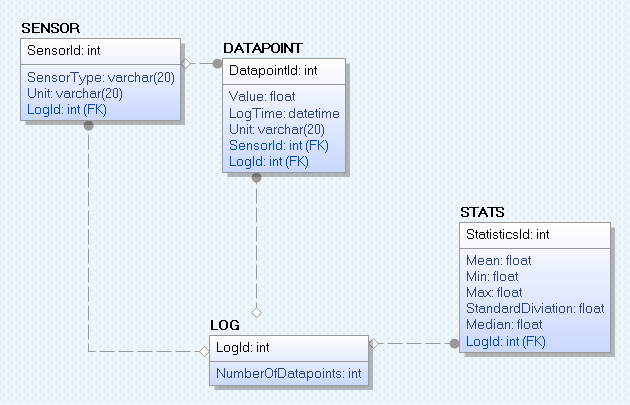
\includegraphics[\width=0.9\linewidth]{Diagrams/SQLDiagram.png}
\caption{The diagram for the SQL database. The database consists of four tables, and the data values are stored in the DATAPOINT table under the column value.}
\label{SQLDiagram}
			\end{figure}
The SENSOR table saves information on the sensor type used, the DATAPOINT table stores information on the datapoints and is connected to the SENSOR table and LOG table. The LOG table stores an amount of numbers connected to each log, such that different loges can be made, and finally the STATS table stores different statistics for the data and is connected with the LOG table. \\
The database also includes a set of stored procedures and triggers, for performing various tasks. The list of these can be seen in figure \ref{PandT}.
			\begin{figure}
\centering
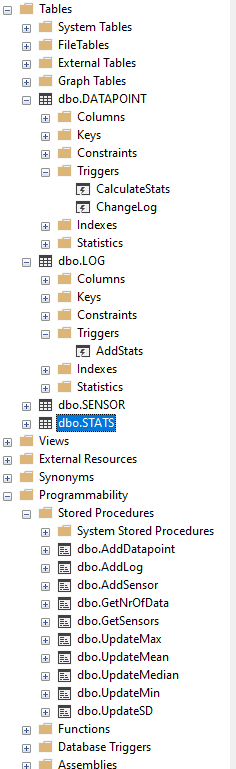
\includegraphics[width=5cm]{Images/ProcessesAndTriggers}
\caption{A list of the tables, stored processes and triggers for the Datalogging and Monitoring System database.}
\label{PandT}
			\end{figure}
		
		\subsection{Datalogging System}
The datalogging system produced in the development environment LabVIEW consists of a main Vi which is diplayed to the user. The gui for this Vi can be seen in figure \ref{Main} and displays the program during a run. The program logs data to the sql server and displays it using a waveform chart.
			\begin{figure}
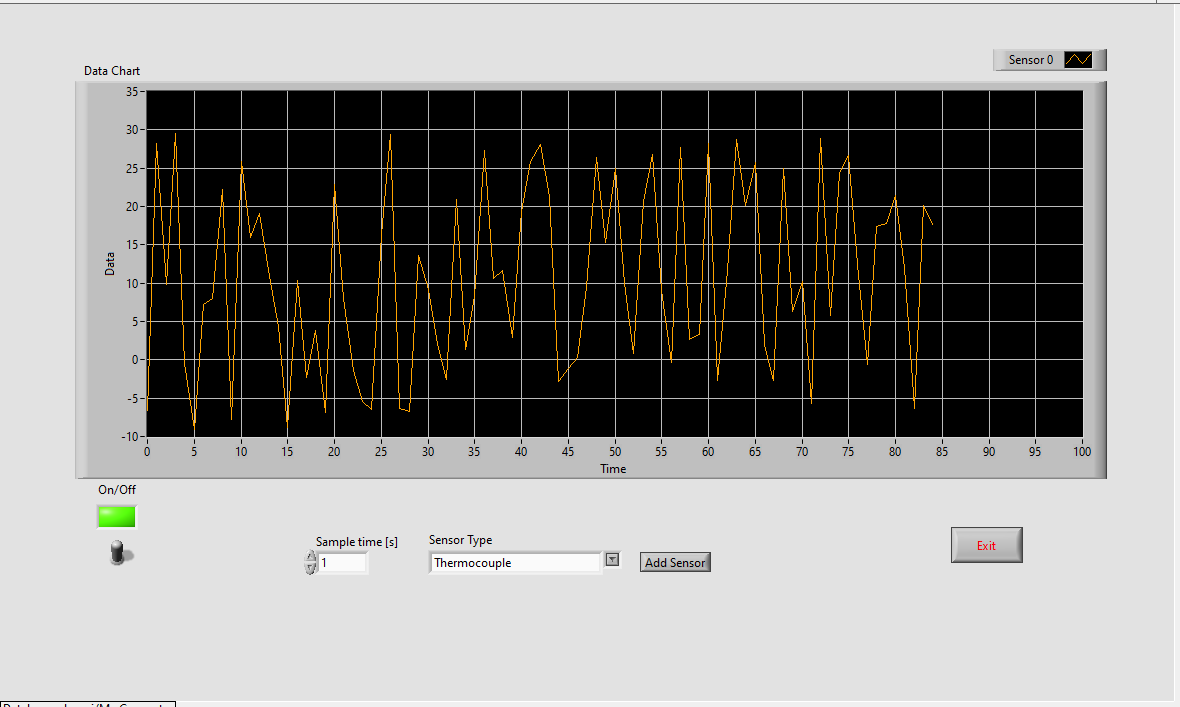
\includegraphics[width=0.9\linewidth]{Images/DaqRunning.png}
\caption{The Datalogging system while running. The program logs a temperature value and displays it to the screen.}
\label{Main}
			\end{figure}
When the program starts, the user is asked to chose the server and database to connect to and the method to connect. Then the program waits for the user to choose a sensor and start the logging. If the required sensor is not already available on the server, the user can click a button to add a sensor and will be asked in a pop up window to provide the new sensors details.

	\section{Discussion}
The system presented doesn't quite solve all the tasks required for the competition, however it does solve the two most important. The SQL database server is capable of storing and providing datapoints and information on the datapoints, and the datalogger can run a simulated temperature sensor while logging the data and display what is logged to a chart. However, there was some technical problems setting up the environment for developing the Monitoring system, and to much time was used on fixing this for there to be enough to actually develop the system. This is obviously something that should be included in the future, and the logging system would also benefit from being able to connect to, log and display multiple sensors at the same time. Finally, a test of the SQL server and the whole system from another device on a local network should also be performed as this would likely be the setup of such a system in the end.

	\section{Conclusion}
The contest was attempted and the produced results fall short of the requirements. The SQL server Does its job at a localhost, and the datalogger is able to log and display the values produced, but there was no time to develop a proper monitoring system.

\printbibliography
	
	\section{Appendix A}
Here you can find the documentation for the SQL database and the datalogging system:
		\begin{figure}[H]
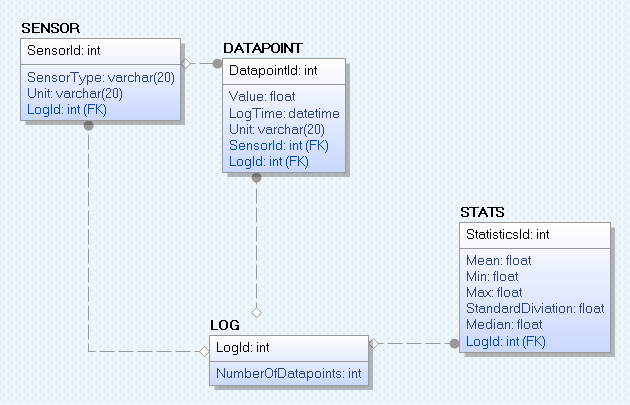
\includegraphics[width=0.9\linewidth]{Diagrams/SQLDiagram.png}
\caption{The diagram for the SQL database. The database consists of four tables, and the data values are stored in the DATAPOINT table under the column value.}
		\end{figure}
		
		\begin{figure}[H]
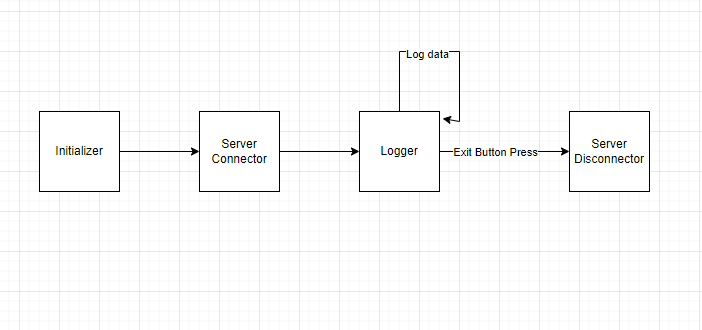
\includegraphics[width=0.9\linewidth]{Diagrams/Logger.png}
\caption{The diagram for LabVIEW DataLogger.}
		\end{figure}

	\section{Appendix B}
All code can be found on the projects GitHub repository \cite{github}.
		\begin{figure}
\centering
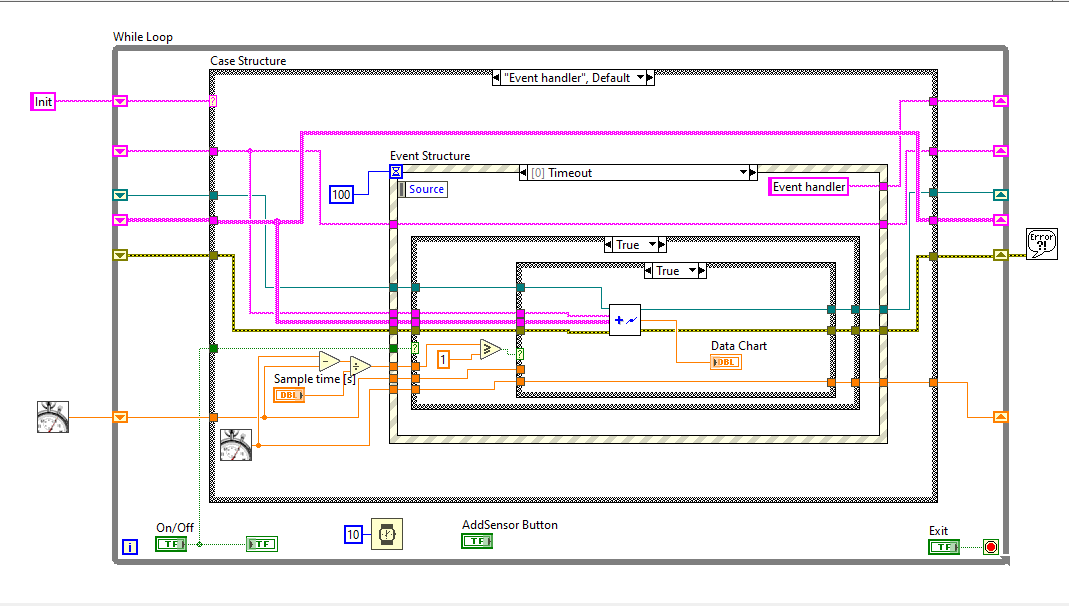
\includegraphics[width=0.7\linewidth]{Images/Logger_Main}
\caption{Code for the Datalogger main window}
		\end{figure}
		\begin{figure}
\centering
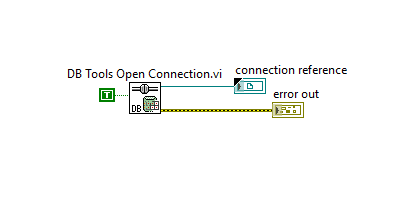
\includegraphics[width=0.7\linewidth]{Images/Logger_connector}
\caption{Code for the connector for the Datalogger}
		\end{figure}
		\begin{figure}
\centering
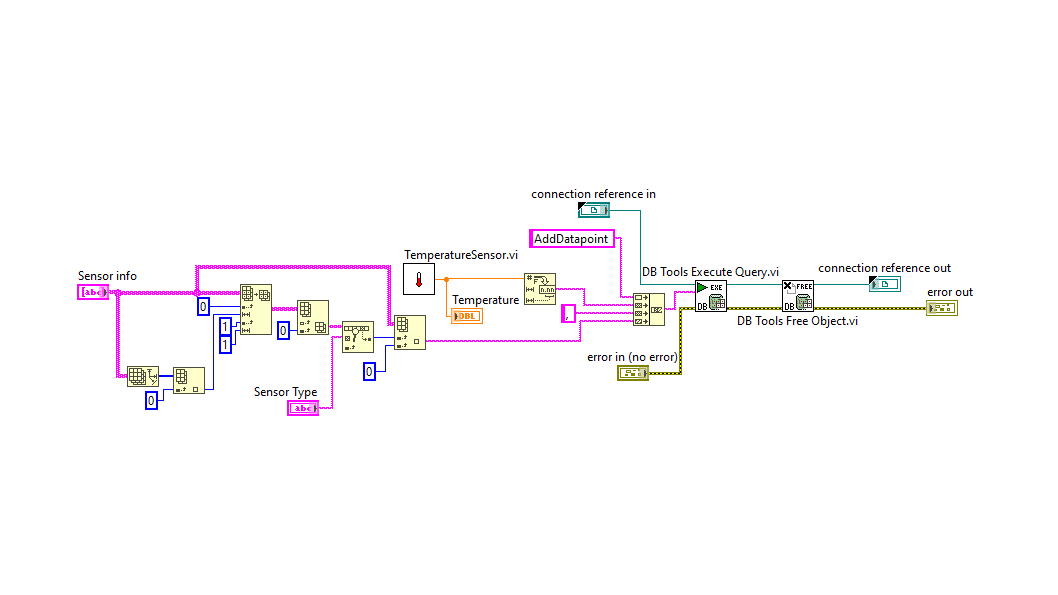
\includegraphics[width=0.7\linewidth]{Images/Logger_datalogger}
\caption{Code for the datalogging part of the datalogger system}
		\end{figure}
		

\end{document}